\lecture{8}{17. September 2025}{Bernoulli Equation Continued}

\subsection{The Bernoulli Equation as an Energy Equation}
The Bernoulli equation, \autoref{eq:berneq}, has been derived by integration of Euler's equation along a streamline for a steady, incompressible, frictionless flow -- I.e. it was derived from the momentum equation for a fluid particle. 

Another equation, that looks almost identical to \autoref{eq:berneq}, although requiring very different restrictions can be obtained from the first law of thermodynamics. 

We consider steady flow in the absence of shear forces. We choose a control volume bounded by streamlines as shown on \autoref{fig:f6_5}, which is often called a \textit{stream tube}.

\begin{figure} [ht]
  \centering
  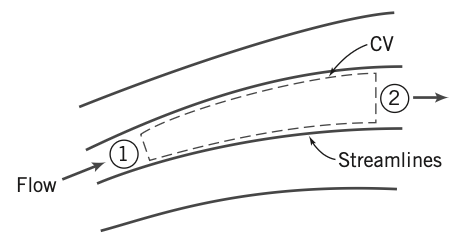
\includegraphics[width=0.5\linewidth]{./figures/f6_5.png}
  \caption{Flow through a stream tube.}
  \label{fig:f6_5}
\end{figure}

We have previously defined the first law of thermodynamics on integral form as
\[ 
\dot{Q} - \dot{W}_s - \dot{W}_{\mathrm{shear}} - \dot{W}_{\mathrm{other}} = \frac{\partial }{\partial t} \int_{\mathrm{CV}} e \rho \, \mathrm{d}V + \int_{\mathrm{CS}} \left( e + pv \right)\rho \textbf{V} \cdot \mathrm{d}\textbf{A}
\]
where
\[ 
e = u + \frac{V^2}{2} + gz
.\]
Under the assumptions mentioned above we have
\begin{itemize}
  \item $\dot{W}_s = 0$,
  \item $\dot{W}_{\mathrm{shear}} = 0$,
  \item $\dot{W}_{\mathrm{other}} = 0$,
  \item steady flow,
  \item and uniform flow and properties at each section.
\end{itemize}

This means that the first law of thermodynamics reduces to
\[ 
\left( u_1 + p_1 v_1 + \frac{V_1^2}{2} + gz_1 \right) \left( - \rho_1 V_1 A_1 \right) + \left( u_2 + p_2 v_2 + \frac{V_2^2}{2} + gz_2 \right) \left( \rho_2 V_2 A_2 \right) - \dot{Q} = 0
.\]
From continuity under the assumptions mentioned above we have:
\[ 
\sum_{\mathrm{CS}} \rho \textbf{V} \cdot \textbf{A} = 0
\]
or
\[ 
\left( - \rho_1 V_1 A_1 \right) + \left( (\rho_2 V_2 A_2 \right) = 0
.\]
I.e.
\[ 
\dot{m} = \rho_1 V_1 A_1 = \rho_2 V_2 A_2
.\]
Also
\[ 
\dot{Q} = \frac{\delta Q}{\mathrm{d}t} = \frac{\delta Q}{\mathrm{d}m} \frac{\mathrm{d}m}{\mathrm{d}t} = \frac{\delta Q}{\mathrm{d}m} \dot{m}
.\]
Therefore, from the energy equation, after rearranging
\[ 
\left( \left( p_2 v_2 + \frac{V_{2}^2}{2} + gz_2 \right) - \left( p_1 v_1 + \frac{V_1^2}{2} + gz_1 \right) \right) \dot{m} + \left( u_2 - u_1 - \frac{\delta Q}{\mathrm{d}m} \right) \dot{m} = 0
\]
or
\[ 
p_1 v_1 + \frac{V_1^2}{2} + gz_1 = p_2 v_2 + \frac{V_2^2}{2}
.\]
If we also assume the flow is incompressible then $v_1 = v_2 = \frac{1}{\rho}$ and,
\[ 
\frac{p_1}{\rho} + \frac{V_1^2}{2} + gz_1 = \frac{p_2}{\rho} + \frac{V_2^2}{2} + gz_2 + \left( u_2 - u_1 - \frac{\delta Q}{\mathrm{d}m} \right)
.\]
We can see that this reduces to the Bernoulli Equation, \autoref{eq:berneq} if the term in parentheses were zero. Therefore if we impose the further restriction,
\[ 
\left( u_2 - u_1 - \frac{\delta Q}{\mathrm{d}m} \right) = 0
,\]
the energy equation reduces to
\[ 
  \frac{p_1}{\rho} + \frac{V_1^2}{2} + gz_1 = \frac{p_2}{\rho} + \frac{V_2^2}{2}+ gz_2 \implies \frac{p}{\rho} + \frac{V^2}{2} + gz = \mathrm{constant}
,\]
which is the Bernoulli equation. 

Here we note that the Bernoulli equation has been derived in two different ways from entirely different frameworks. It may seem that the restriction, relating heat transfer and internal thermal energy change, is needed for the energy equation to transform to the Bernoulli equation.  However, for an incompressible and frictionless flow without shear forces, heat transfer results only in a temperature change and does not affect neither pressure nor velocity. 

\subsection{Energy Grade Line and Hydraulic Grade Line} \label{sec:egl}
For a steady, incompressible, frictionless flow we may use the Bernoulli equation, \autoref{eq:berneq}:
\[ 
\frac{p}{\rho} + \frac{V^2}{2} + gz = \mathrm{constant}
.\]
If we divide this by $g$ we obtain another form
\[ 
\frac{p}{\rho g} + \frac{V^2}{2g} + z = H
.\]
Here $H$ is called the \textit{total head} of the flow and is a measure of the total mechanical energi in units of meters. In a fluid flow $H$ will not be constant but will instead continuously decrease as mechanical energy is converted to thermal. A useful graphical approach is to define this to be the \textit{energy grade line} (EGL),
\[ 
\mathrm{EGL} = \frac{p}{\rho g} + \frac{V^2}{2g} + z
.\]
We can also define the \textit{hydraulic grade line} (HGL),
\[ 
\mathrm{HGL} = \frac{p}{\rho g} + z
.\]
From these we get
\[ 
\mathrm{EGL} - \mathrm{HGL} = \frac{V^2}{2g}
,\]
i.e. the difference between the EGL and HGL is the dynamic pressure term. The function of this is shown graphically on \autoref{fig:f6_6}. Here it is worth noting that for incompressible, inviscid flow without work devices the EGL is constant. Furthermore, the HGL will always be lower than the EGL by distance $\frac{V^2}{2g}$. 

\begin{figure} [ht]
  \centering
  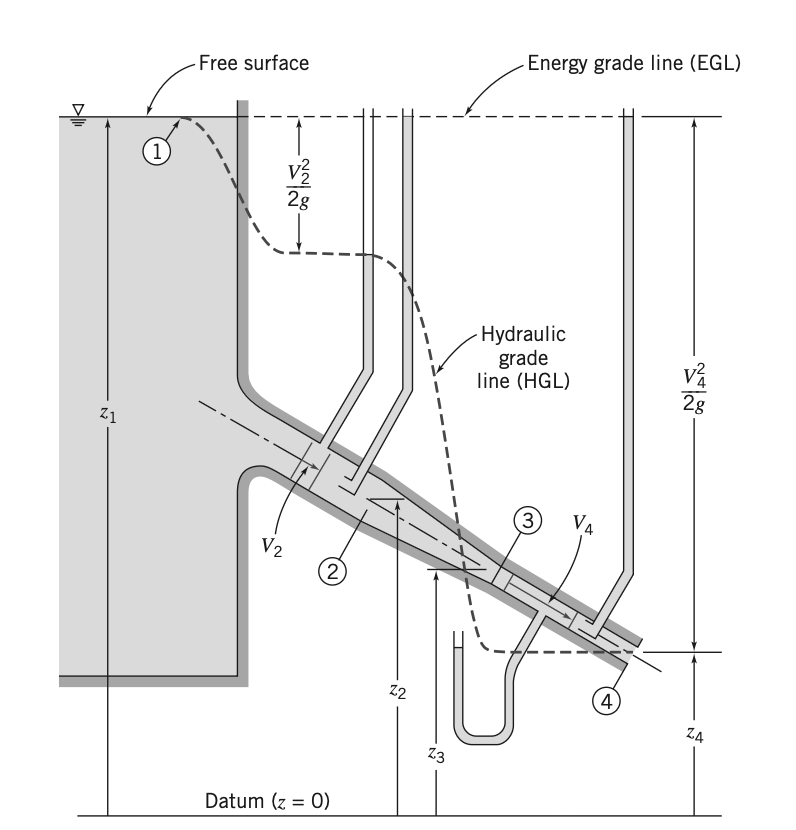
\includegraphics[width=0.5\linewidth]{./figures/f6_6.png}
  \caption{Energy and hydraulic grade lines for frictionless flow}
  \label{fig:f6_6}
\end{figure}


\subsection{Unsteady Bernoulli Equation: Integration of Euler's Equation Along a Streamline}
The Bernoulli equation need not be restricted by the assumption of steady flow. The momentum equation for frictionless flow can be written (with $\textbf{g}$ in the $-z$ direction) as
\[ 
\frac{\mathrm{D}\textbf{V}}{\mathrm{D}t} = - \frac{1}{\rho} \nabla  p - g \hat{k}
.\]
This is a vector equation, which can be converted to a scalar equation by taking the dot product with $\mathrm{d}\textbf{s}$, where $\mathrm{d}\textbf{s}$ is an element of distance along a streamline. Thus
\[ 
\frac{\mathrm{D}\textbf{V}}{\mathrm{D}t} \cdot \mathrm{d}\textbf{s} = \frac{\mathrm{D}V}{\mathrm{D}t} \, \mathrm{d}s = V \frac{\partial V}{\partial s} \, \mathrm{d}s + \frac{\partial V}{\partial t} \, \mathrm{d}s = - \frac{1}{\rho} \nabla p \cdot \mathrm{d} \textbf{s} - g \hat{k} \cdot \mathrm{d} \textbf{s}
.\]
Here we note that
\begin{align*}
  \frac{\partial V}{\partial s} \, \mathrm{d}s &= \mathrm{d}V & &(\text{the change in } V \text{ along }s)\\
  \nabla p \cdot \mathrm{d}\textbf{s} &= \mathrm{d}p & &(\text{the change in pressure along }s) \\
  \hat{j} \cdot \mathrm{d}\textbf{s} &= \mathrm{d}z & &(\text{the change in }z \text{ along }s)
.\end{align*}
Substituting these into the expression we obtain
\[ 
V \, \mathrm{d}V + \frac{\partial V}{\partial t} \, \mathrm{d}s = - \frac{\mathrm{d}p}{\rho} - g \, \mathrm{d}z
.\]
Integrating this along a streamline from a point, 1, to another point, 2, yields
\[ 
\int_{1}^{2} \frac{\mathrm{d}p}{\rho} + \frac{V_2^2 - V_1^2}{2} + g \left( z_2 - z_1 \right) + \int_{1}^{2} \frac{\partial V}{\partial t} \, \mathrm{d}s = 0
.\]
For incompressible flow, $\rho = \mathrm{constant}$, and the above equation then reduces to
\[ 
\frac{p_1}{\rho} + \frac{V_1^2}{2} + gz_1 = \frac{p_2}{\rho} + \frac{V_2^2}{2} + gz_2 + \int_{1}^{2} \frac{\partial V}{\partial t} \, \mathrm{d}s
.\]
This is applicable for incompressible, frictionless flow along a streamline. This is also known as the Bernoulli equation for unsteady flow. It differs from the Bernoulli equation by the term $\int_{1}^{2} \frac{\partial V}{\partial t} \, \mathrm{d}s$. This term can be interpreted as the work involved in the rate of increase of momentum of the fluid on the streamline over time, as opposed to the change in momentum over distance, represented by the change in velocity from $V_1$ to $V_2$.


\subsection{Irrotational Flow}
Irrotational flows were briefly mentioned in \autoref{sec:rot}. These are flows in which the fluid particles do not rotate ($\boldsymbol{\omega} = 0$). The only stresses that can generate particle rotation are shear stresses. Therefore, all inviscid flows are inherently irrotational unless the particles were somehow initially rotating. The irrotationality condition is
\[ 
\nabla \times \textbf{V} = 0 \implies \frac{\partial w}{\partial y} - \frac{\partial v}{\partial z} = \frac{\partial u}{\partial z} - \frac{\partial w}{\partial x} = \frac{\partial v}{\partial x} - \frac{\partial u}{\partial y} = 0
.\]

\subsubsection{Bernoulli Equation Applied to Irrotational Flow}
The Bernoulli equation has been shown to hold along a streamline for a steady, incompressible, inviscid flow. If in addition to this, the flow field is also irrotational (i.e. the particles had no initial rotation), such that $\nabla  \times \textbf{V}= 0$, then Bernoulli's equation will be the same value for all streamlines -- this means that for irrotational flows the Bernoulli equation is also valid across different streamlines.

To show this we start with Euler's equation in vector form,
\[ 
\left( \textbf{V} \cdot \nabla  \right) \textbf{V} = - \frac{1}{\rho} \nabla p - g \hat{k}
.\]
Using the vector identity 
\[ 
\left( \textbf{V} \cdot \nabla  \right)\textbf{V} = \frac{1}{2} \nabla  \left( \textbf{V} \cdot \textbf{V} \right) - \textbf{V} \times \left( \nabla  \times \textbf{V} \right)
,\]
we see that for irrotational flow, when $\nabla  \times \textbf{V} = 0$,
\[ 
\left( \textbf{V} \cdot \nabla  \right) \textbf{V} = \frac{1}{2} \nabla  \left( \textbf{V} \cdot \textbf{V} \right)
\]
hence Euler's equation for irrotational flow can be written as
\[ 
\frac{1}{2} \nabla  \left( \textbf{V} \cdot \textbf{V} \right) = \frac{1}{2} \nabla \left( V^2 \right) = - \frac{1}{\rho} \nabla p - g \hat{k}
.\]
We consider an arbitrary displacement from $\textbf{r}$ to $\textbf{r} + \mathrm{d}\textbf{r}$ not necessarily along a streamline. Taking the dot product of this with each term in the above yields
\[ 
\frac{1}{2} \nabla \left( V^2 \right) \cdot \mathrm{d}\textbf{r} = - \frac{1}{\rho} \nabla p \cdot \mathrm{d}\textbf{r} - g \hat{k} \cdot \mathrm{d}\textbf{r}
\]
hence
\[ 
\frac{1}{2} \mathrm{d}\left( V^2 \right) = - \frac{\mathrm{d}p}{\rho} - g \, \mathrm{d}z
\]
or
\[ 
\frac{\mathrm{d}p}{\rho} + \frac{1}{2} \mathrm{d}\left( V^2 \right) + g \, \mathrm{d}z = 0
.\]
Integrating this for an incompressible flow gives
\[ 
\frac{p}{\rho} + \frac{V^2}{2} + gz = \mathrm{constant}
\]
which is the Bernoulli equation. Therefore it has been shown that this holds between any two general points in an irrotational flow. 
